\documentclass{article}
\title{Project 3 \\ FYS-STK3155/4155}
\author{Magnus Bergkvam}
\usepackage{url}
\usepackage{amsmath}
\usepackage{graphicx}
\usepackage{subfig}
\usepackage{bm}
\usepackage{listings}

\graphicspath{{../figures/}}


\begin{document}
\maketitle
\bibliographystyle{unsrt}

\section{Abstract}
Machine learning classifiers have many important uses, from spam classification
of emails, to image classification in the medical sector and much more. They
also have found use for quite important and high-risk tasks like credit-card
fraud detection \cite{creditcardfraud}, where a good classifier is important
for as many credit-card frauds to be stopped as possible, while at the same
time legitimate payments going through.

In this project we explored how different models performed on a data-rich
credit-card fraud dataset \cite{kaggleccdata}. For this we looked at three
different types of models, one being a simple logistic regression, another one
being neural networks and finally we looked at gradient-boosted decision trees.
Unlike the previous projects we have just used established machine-learning
libraries namely sklearn, tensorflow and xgboost for the models and done
parameter tuning on each of the models. What we found was that the logistic
regression did manage to classify most predictions at $96\%$ overall accuracy
on the test-data, however it still performed considerably worse than the other
two models. For the neural network we ended up with a model with two hidden
layers, each with $100$ nodes, using the RMSProp optimizer, with some $l_2$
regularization and relu activation functions. The neural network did give us
quite good classification with it being able to correctly classify all the
fraud cases, and only giving $62$ false positives out of more than $35 000$
observations. The best performance though was the gradient boosted decision
tree, also correctly classifying all the fraud cases and only giving $21$ false
positives.

Overall this project has shown that for credit card fraud detection, gradient
boosting especially, but also neural networks, are both very good classifiers
for this task. This effect likely translates into other data-rich binary
classification cases as well.

\section{Introduction}
Credit card fraud detection is one of many application where machine learning
binary-classification models are widely used. Furthermore it is a case where
having a good classifier is essential for the credit-card system to work in the
first place. It is important that the vast majority of legitimate purchases are
detected as legitimate as reliability of use of credit cards is quite important
if you want people to use your credit cards. For example, when going to the
store and buying something you shouldn't have to worry at all about the card being
declined. At the same time it is perhaps even more important that the actual
frauds are detected as such, as the credit-card company can then take action to
block the payments and maybe even the card. This is both important for the user
of the credit card and the issuer, as it can be a huge hurdle for the owner if
fraud payments are not detected and go through normally, which is both
uncomfortable and time-consuming. Additionally for the issuer, the more fraud
payments they let go through, the more payments they potentially have to cover
themselves.

What is clear is then that a very good classifier is needed in order to limit
these situations discussed. We will here try to explore some different models
for classifying fraud and see how good they perform. The dataset we will be
using contains more than $550 000$ transactions, each with $28$ anonymized
features plus the amount spent, and a binary response representing fraud or not
fraud. We will focus mainly on three types of models. The simplest one being
logistic regression, then we will go back to neural networks as we found that
they performed very well in project 2 \cite{githubrepoproject2} and finally
we'll look at a decision tree, more specifically a gradient boosting tree.

A motivation behind using logistic regression is that as we have already seen,
they often can perform rather well on less complex problems, due to their low
complexity (low variance). On problems like these this usually can't compete
with the other two models, but we will see how big of a gap we'll get between
them, and this can also serve as some sort of benchmark for the other two
models. Neural networks is a good choice for a lot of problems, with them being
very general and often perform well when we have a lot of data. Boosting trees
we have chosen to bring in here because they very often are a go-to for
classification purposes, with them being the winner of many classification
competitions. Additionally they are more intuitive than the neural network
approach, and less computationally expensive.

We'll first in the method introduce some of the models we'll use, and go
through the data a bit closer, before we look at how the three different models
perform, and from there on we will try to conclude which of the three models
performs the best for this data and try to put into perspective just how good
they perform, and if it is good enough.

\section{Methods}
\subsection{The credit card fraud data}
At the heart of all our experimentation is the credit-card fraud detection
data from 2023 \cite{kaggleccdata}. This is a dataset where each observation
corresponds to one transaction. Luckily for our predictions as well, this is
quite rich on data with there being $568630$ total observations/transactions.
Furthermore this data is equally split among the two classes, with there being
$284315$ non-fraudulent and fraudulent transactions each. This is probably
going to be a good thing for our models, as the models has then as much
information of what constitutes a fraudulent transaction, as a non-fraudulent
transaction.

The data is collected using transactions from European credit card holders in
the year $2023$ \cite{kaggleccdata}. The fact that we only have data collected
from Europeans does perhaps limit the performances of our models on
non-european card holders. If for example in another part of the world a
legitimate credit-card transaction typically looks different, or likewise with
fraud, our models are not guaranteed to be as good classifiers as the ones we
will get from this dataset, so this is something we will need to keep in mind.
Each transaction contains a unique identifier (labeled id), $28$ anonymized
features (labeled $\text{V}1$ to $\text{V}28$), the transaction amount (labeled
as Amount) and a categorical variable indicating whether we have a fraudulent
transaction (labeled as Class). For the Class we have that $1$ constitutes
fraud while $0$ constitutes a legitimate transaction. We will obviously not use
id id for training here, as this should not impact whether a transaction is
fraudulent, but we will use all the other variables in our models, with Class
as the binary response. Another thing which makes this data quite convenient is
that all of the features are numerical, with there being no NA/NULL values as
all, which makes the required preprocessing here very small (the only
preprocessing I'll do is scaling the rows with StandardScaler).
\\

To see some dependencies of the response for each explanatory variable we can
create a box-plot for each feature. Figure \ref{databoxplot} shows exactly
this. As we can see there are quite a few of the anonymized features especially
which looks to be distributed slightly differently for the fraudulent
transactions than the legitimate ones. This difference in distribution of some
of the features looks promising our classification.


\begin{figure}
	\centering
	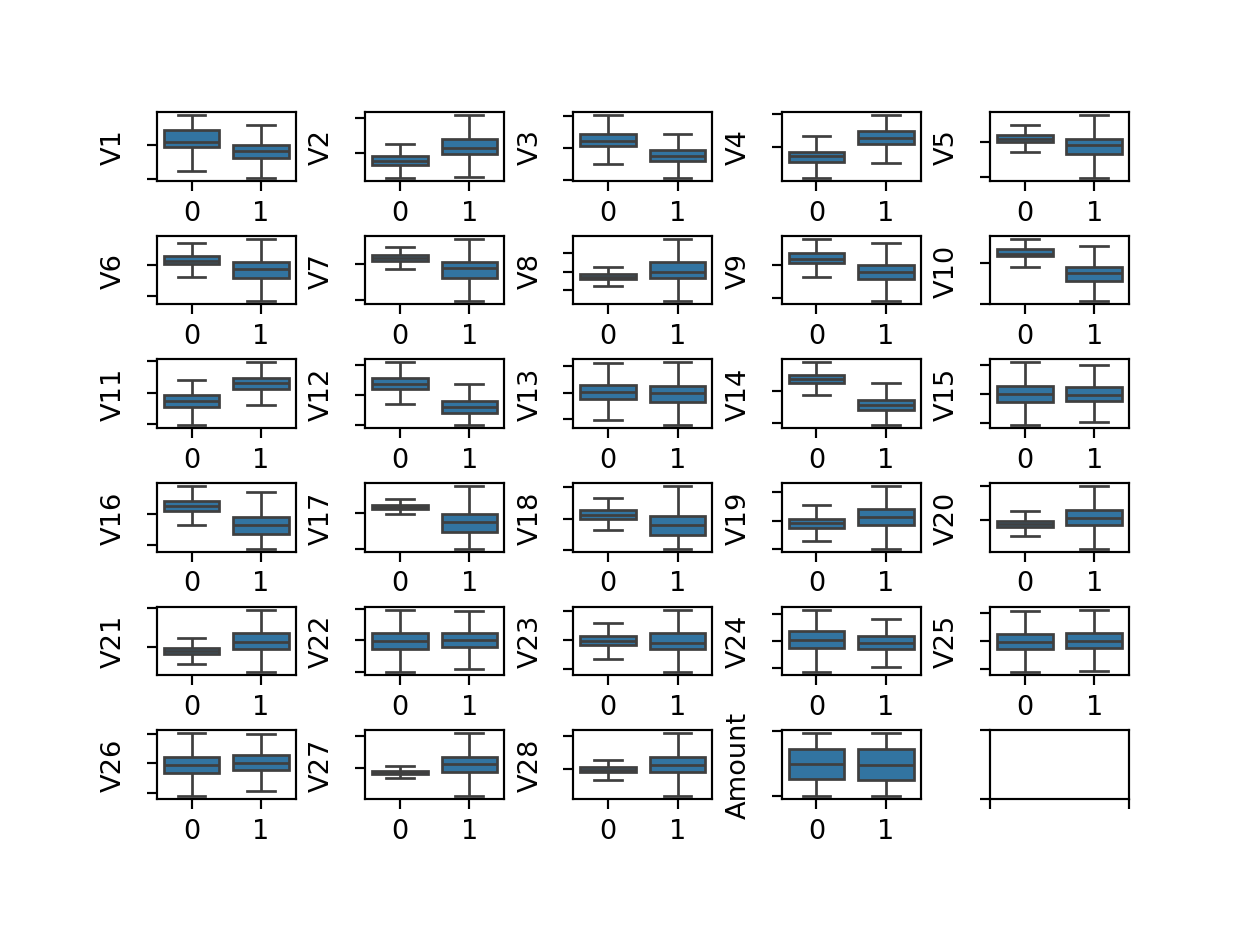
\includegraphics[scale=0.8]{data_features_boxplot}
	\caption{Shows a boxplot with each feature along the y-axis and the
		binary response on the x-axis. This plot was generated from a random
		sample of $10 000$ observations of the data. We see that for the anonymized
		features (bar 13 15 22 23 24 25 26) there seems to be a clear difference in
		distributions for the feature-values for the non-fraudulent and fraudulent
		transactions.}
	\label{databoxplot}
\end{figure}


\subsection{Logistic regression}
The first and most simple method we will explore is the logistic regression. I
will not go into detail on this method here, as this already has been presented
in project 2 \cite{githubrepoproject2}. We will here simply do a train-test
split and train a logistic regression on the training-set and evaluate the
performance on a test-set. For the features we will first try a model with just
the features directly from the dataset, and then try with polynomial features
of second degree polynomials (with interactions). We will not add a higher
polynomial-degree than this due to the fact that we have $29$ features already and
a high polynomial order will give us considerably more features, which can both
lead to overfitting, and to problems with memory (keep in mind that the dataset
here is quite big). For finding the appropriate regularization parameter we
will here take use of cross-validation. Here we will simply use the
LogisticRegressionCV which does most of the job for us.

\subsection{Neural Networks}
For the neural networks in this project we will use a basic multi-layer
perceptron, this time using tensorflow. I will assume knowledge of the basic
setup of training, and. For more details on the neural networks feel free to
check out the report of project 2 \cite{githubrepoproject2}. We will spend some
time tweaking the based on the performance based on what gives us good
performance on the validation set. Luckily for us we have a lot of data, with
the two classes being quite evenly distributed, so using this approach over
something like corss-validation should be unproblematic.

The main things we will be tweaking is the regularization parameter (we will
limit ourselves to use $l_2$ regularization), the optimization method (with the
corresponding learning-rate), the activation functions and the network size.
For this we will use a greedy method, starting with determining the optimal by
testing a grid of learning-rates and regularization parameters, before we then
explore the activation functions using this method, again testing with a grid
of learning-rates and regularization parameters, before we lastly try different
hidden layer sizes for the chosen method and activation function now testing on
a grid of different learning-rates and keeping the best learning-rate
previously determined. The output function will be fixed to be the sigmoid
function in this case as we are dealing with binary classification, while the
cost-function will be binary cross-entropy, both just as in project 2.

The optimization methods we will try in this case is just as in project 2, i.e.
AdaGrad, Adam, RMSProp and SGD. We have dropped trying out normal gradient
descent, because of it's uncompetitive performance in project 2, as well as the
fact that our dataset now will be huge, meaning that the amount of epochs we
are willing to give in the learning-process is severely limited, meaning it
should have even worse prerequisites in this case. All these are built directly
into tensorflow so the amount we need to implement here is quite limited.

For the activation-functions we will try out the relu and sigmoid (which we
already have explored in project 2), as well as some other activation functions
built into tensorflow. Notably these are swish, tanh and elu. We will now go a
little bit into these:
\subsubsection{tanh}
The tanh is given by:
$$\text{tanh}(x) = \frac{\exp(x) - \exp(-x)}{\exp(x) + \exp(-x)}$$ \cite{wikihyperbolicfunctions}
This looks much like the sigmoid function, in that is has the same s-shape, but
is different in the sense that the sigmoid limits us between $0$ and $1$, while
the tanh limits us between $-1$ and $1$. This can in some situations be
preferable.

\subsubsection{swish}
The swish is given by:
$$\text{swish}(x) = x \cdot \text{sigmoid}(x).$$ \cite{tensorflowdocswish}
Using our knowledge about the sigmoid-function we see that as $x$ grows, the
sigmoid will approach $1$ quite quickly. This means that for high values of
$x$, the function will behave much like the relu. For negative values of $x$ we
have that the sigmoid becomes very close to $0$, much quicker than the linear
function $x$ grows towards $-\infty$, so the product will be very close to $0$,
again much like the relu. However for small absolute values we will get a
shrinking in absolute value of the activations. This function often works
better than the ReLU on deep models on challenging datasets
\cite{ramachandran2017searching}, so we will explore if this is one of those
cases.

\subsubsection{ELU}
The exponential linear unit is given by:
$$\text{elu}(x) = \begin{cases} x \qquad \qquad & \text{if}\ \ x > 0 \\ \alpha \cdot (\exp(x) - 1) & \text{if}\ \ x < 0 \end{cases}.$$ \cite{tensorflowdocelu}
We will here just use $\alpha = 1$ (which is the default), but of course it is
easy to test others as well. The ELU can lead to faster learning and better
performance on neural nets with more than $5$ layers in particular
\cite{clevert2016fast}, which is less than what we will be using here,
but we will try it anyway because including this takes essentially no code.

\subsection{Boosting trees}
This is a method we haven't been through earlier, so we'll go a little bit more
into this here. At the core of a boosting-tree is a normal classification-tree
which we will use as a so-called weak classifier. We will first look a little bit into how this method works.

\subsubsection{Classification trees}
A classification tree is a rather simple. Like other decision trees they are
typically divided into a root node, interior nodes and leaf nodes. The nodes
are connected via branches, where the branch we move along with being dependent
on a test on the node we are in, where the test has only two outcomes. Each of
the leaf nodes contains the classification we should make
\cite{lecturesweek46}. To make predictions on a tree we start at the root
node and then move along the branch according to the test at the root-node
until we come to a new node, where we do the same procedure until we end up at
a leaf node, in which case we have our prediction.

For finding appropriate structure of the tree (that is the appropriate tests
and nodes), perhaps the most popular algorithm is the CART algorithm. This uses
what is called the Gini index, which we will denote $G$. Let $p_{m 1}$ be the
proportion of observations of credit card fraud (i.e. with $y_i = 1$) within a
region $R_m$ and $p_{m 0} = 1 - p_{m 1}$ be the proportion of non-fraud cases
within $R_m$. More formally we have:
$$p_{m 1} = \frac{1}{N_m} \sum_{x_i \in R_m} I(y_i = 1).$$
The Gini index is then:
$$G = \sum_{i=0}^{1} (p_{m i} (1 - p_{m i})) = 2 p_{m 1} (1 - p_{m 1}).$$
This Gini index gives us a metric of how good each split is. A higher
Gini-index means that region $R_m$ contains a higher proportion of one class,
which means we have managed to find criterion which hopefully accurately is
able to classify observations of the classes. The Cart algorithm is one way of
optimizing with regards to this gini-factor. This algorithm splits the data
into two subsets by doing a split on a single feature $k$ and a threshold $t_k$
\cite[s.~The CART algorithm for Classification]{lecturesweek46}. This is done
by searching for the $(k, t_{k})$ which minimizes the cost:
$$C(k, t_k) = \frac{m_{left}}{m} G_{left} + \frac{m_right}{m} G_{right}$$
, where $m_{left}$ is the amount of observations in the left region $m_{right}$
is the amount of observations in the right region, $m$ is the amount of
observations in the region we are doing the split on, and $G_{left}$ and
$G_{right}$ is the Gini in left and right subregion. A lower value of $C(k,
	t_k)$ essentially means that the overall split results in more pure regions.
Finding this exact $(k, t_k)$ may involve searching through all the features
and then for each feature find the $t_k$ by searching through a lot of
thresholds and then choosing the optimal pair $(k, t_k)$.

\subsubsection{Gradient Boosting}
While normal classification trees will be able to fit the training data well,
they often will lead to overfitted trees if we fit the training-data too well,
and many of the techniques to combat overfitting will often lead to trees not
giving that good performance. Predictions on new data often will not be very
good because of this. However, they will often be able to pick up some
underlying patterns in the data, more so than just making random predictions
anyway. This enables its use as a weak learner for a boosting setting. In
gradient boosting we combine many weak learners, adding them together to create
a good learner. For gradient boosting, assume we have a cost-function function
$C(f) = \sum_{i=0}^{n-1} L(y_i, f(x_i))$, where $f$ is our classifier. We then
have the following algorithm \cite[s.~Gradient Boosting,
	algorithm]{lecturesweek46}:
\begin{itemize}
	\item Initialize our estimate $f_0(x)$ (this will be our classification tree)
	\item for $m = 1, 2, \dots, M$ do:
	      \begin{itemize}
		      \item Compute the negative gradient vector $\bm{u}_m = -\frac{\partial C(\bm{y}, \bm{f})}{\partial \bm{f}(x)}$ at $f(x) = f_{m - 1}(x)$.
		      \item Fit the base-learner (again is this is a classification tree) to this negative gradient $h_m(u_m, x)$.
		      \item Update the estimate $f_m(x) = f_{m-1}(x) + h_m(u_m, x)$.
	      \end{itemize}
\end{itemize}.
We then will get a final classifier $f_M$. For our loss-function in a
binary classification case we could for example use:
$$C(\bm{y}, \bm{f}) = \sum_{i=0}^{n-1} \exp(-y_i (f_{m-1}(x_i) + \beta G(x_i))) = \sum_{i=0}^{n-1} w_i^m \exp(-y_i \beta G(x_i))$$
, where $y_i$ is $-1$
if we do not have fraud and $1$ if we do have fraud, $\beta$ is the weighted
parameter which we want to optimize and $G$ is our weak classifier. The XGBoost
(Extreme Gradient Boosting) python library, builds upon the idea of gradient
boosting and makes optimizations on top of this in many ways. Often gradient
boosted trees are very good for classification purposes.

\section{Results}
\subsection{Logistic regression}
In \textbf{lr\_creditcard.py} in the project codes \cite{githubrepoproject3} we
have tested three different models, two of whom are fitted with the ordinary
features, with $l_1$ and $l_2$ regularization, and then a logistic
regression-model with polynomial features. Table \ref{lrresults} shows the
results for the three different models. Here we can see that the choice of
regularization type does not give any meaningful difference for performance,
but that the model with second degree polynomial features performing a lot
better. Figure \ref{lrconfusionmats} and \ref{lrpolyconfusionmat} shows
the confusion matrices for the models without polynomial features and with
polynomial features respectively. We see that for the polynomial feature model
this gave , which is overall quite good, but perhaps not as good as what we
would wish for as this means around $\frac{249}{70903+249} \approx 0.35\%$ of
non-fraud cases are detected as fraud, while $\frac{148}{70858 + 148} \approx
	0.21\%$ of actual fraud cases are not detected as such. Furthermore figure
\ref{lrroccurves} shows a ROC-curve for the models not using polynomial
features. Here we see that the ROC-curve is quite good, so we could adjust the
classification-boundary to minimize the false positives without getting too
many true negatives and vice versa. If we were to look at the ROC-curve for the
polynomial model this would be near perfect, which allows for the same
possibility of adjusting the classification boundary here as well.

\begin{figure}
	\centering
	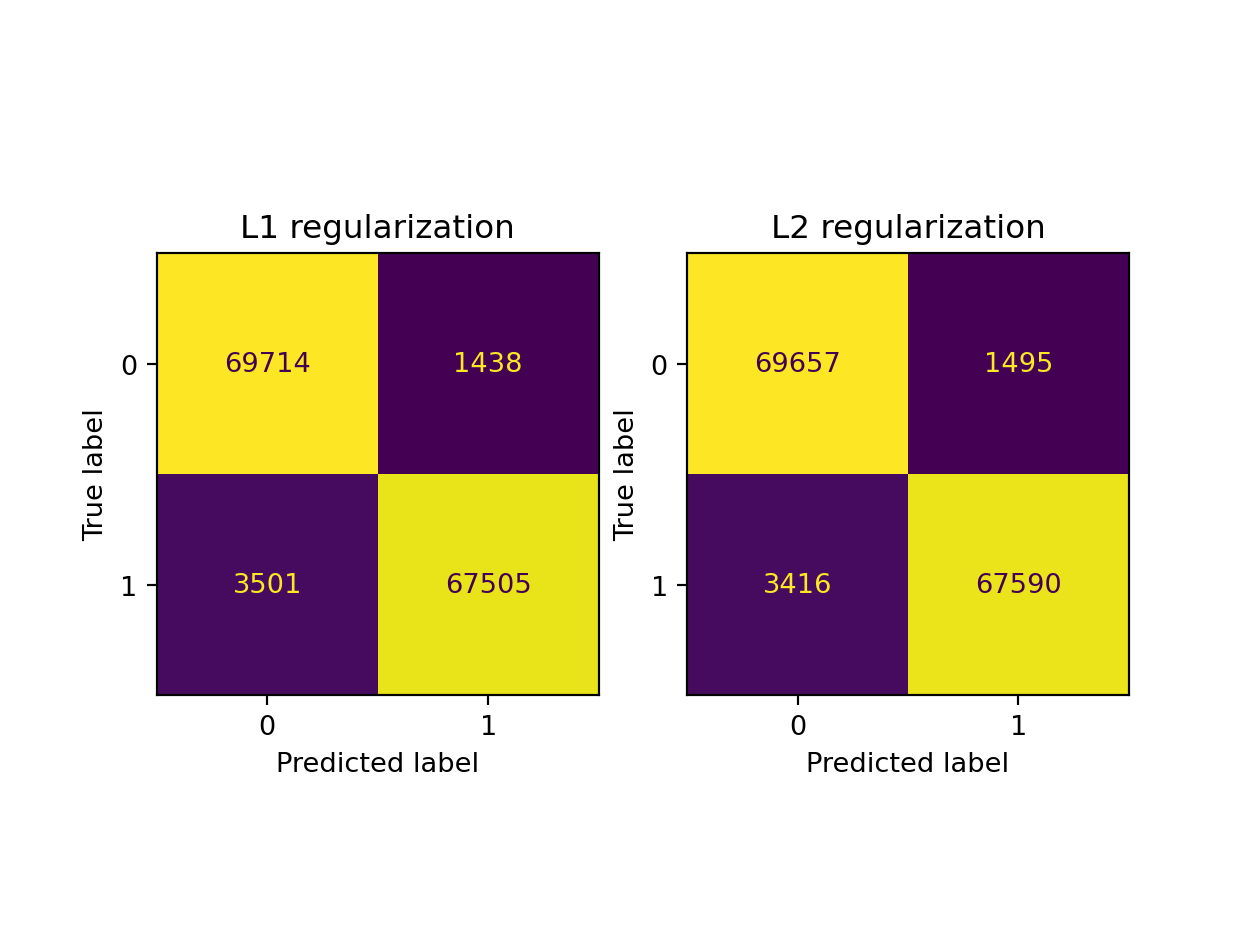
\includegraphics[scale=0.8]{lr_confusion_mat}
	\caption{Shows the confusion matrices for a logistic-regression with
		$l_1$ and $l_2$ regularization, with the regularization-parameter
		determined through cross-validation.}
	\label{lrconfusionmats}
\end{figure}

\begin{figure}
	\centering
	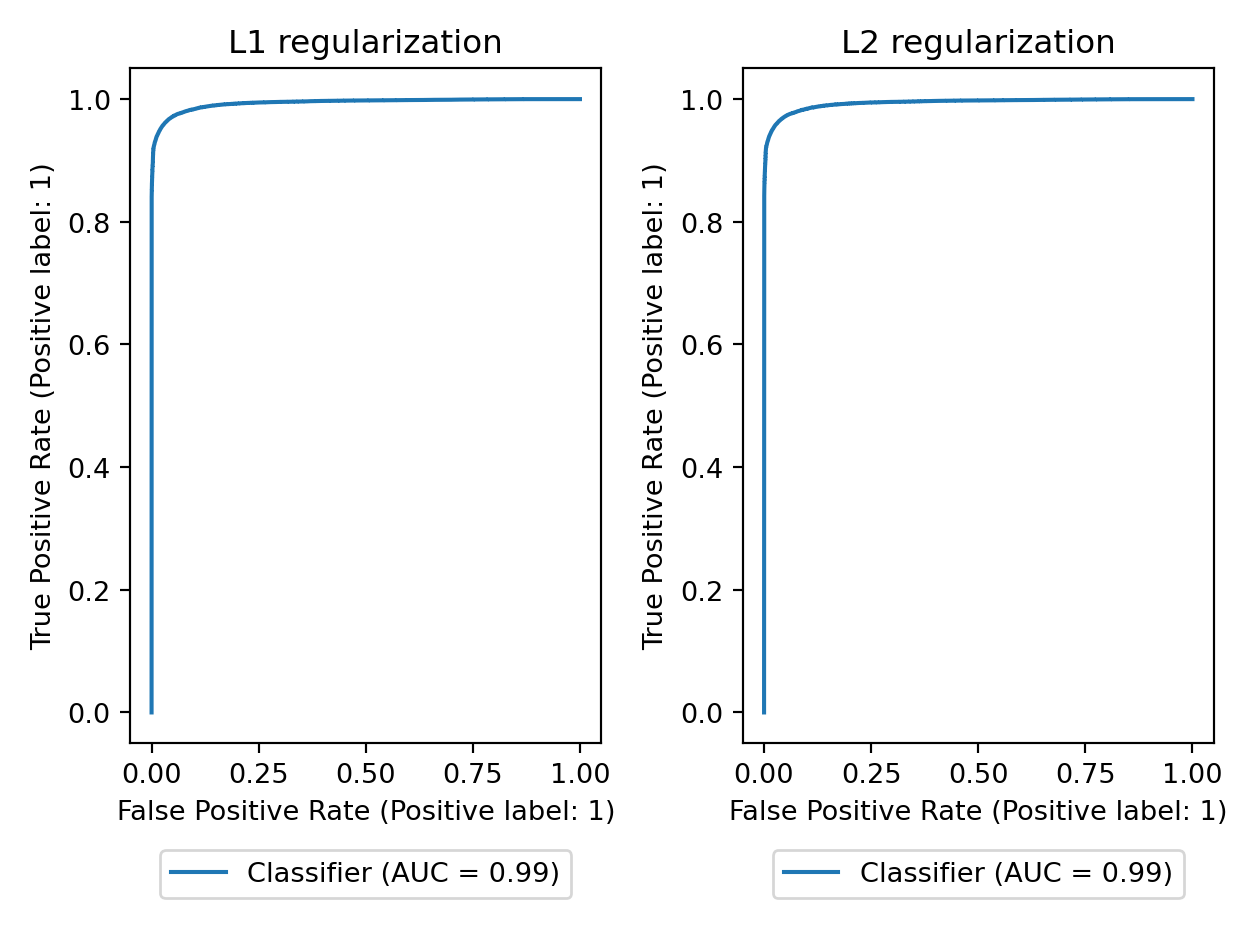
\includegraphics[scale=0.8]{lr_roc_curve}
	\caption{Shows the ROC-curve for a logistic-regression with
		$l_1$ and $l_2$ regularization, with the regularization-parameter
		determined through cross-validation.}
	\label{lrroccurves}
\end{figure}

\begin{figure}
	\centering
	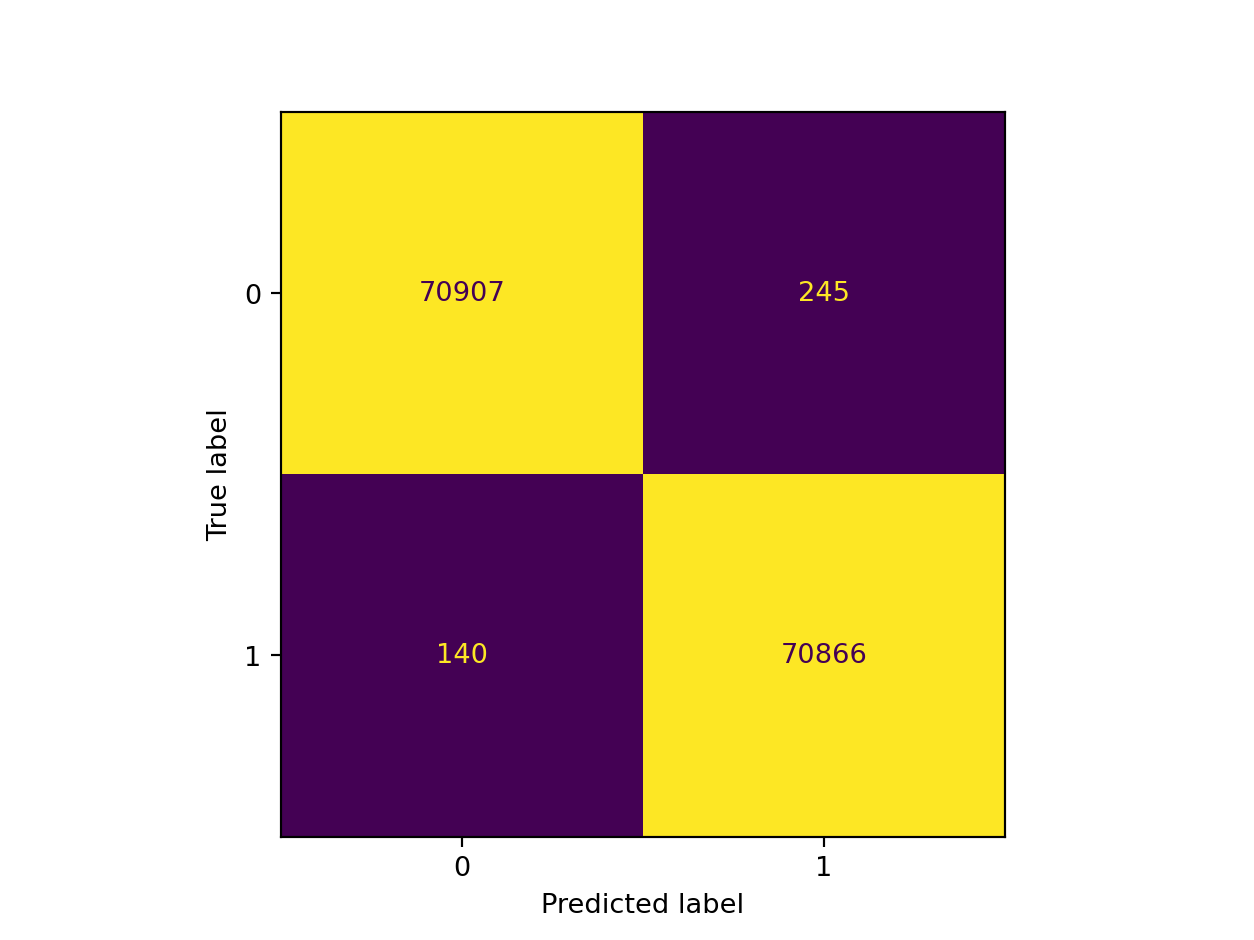
\includegraphics[scale=0.8]{lr_poly_confusion_mat}
	\caption{Shows the confusion matrix for a logistic-regression with
		$l_2$ regularization, with the regularization-parameter
		determined through cross-validation, and using polynomial
		features of degree $2$.}
	\label{lrpolyconfusionmat}
\end{figure}

\subsection{Neural networks}
The \textbf{nn\_creditcard.py} program explores fitting neural networks to the
credit-card data. Table \ref{nnmethodres} shows the accuracy on the
training-data ran on a single epoch over some smaller training-dataset. Here we
see that the different methods give essentially the same results. The
optimization method here therefore doesn't seem to matter all that much for the
performance on new data. Which optimizer we choose will therefore not matter
too much. To see more about how the accuracy variaes depending on the
learning-rate and regularization-parameters, see figure \ref{nntestacchm}. For
the results afterwards we therefore have just moved picked RMSProp as our
method of choice forwards. Looking at the results this may seem odd as this
didn't give the absolute highest accuracy for our results, but keep in mind
that tensorflow is not built with complete determinism in mind, so the results
will vary from each time you run the program, and on another occasion this
performed the best. After choosing this model we explored the different
activation functions. Table \ref{nnactivres} shows the accuracy on the
test-data for the different models. Here we see a more substantial difference,
where relu did seem to perform the best by a little margin. Our model then
becomes a RMSProp with relu activation functions, with the optimal
regularization parameter occurring at $\lambda = 10^{-5}$ and the best
learning-rate being $\eta = 10^{-\frac{5}{2}}$. Having found this we also try
some different layer-sizes for the neural network. Table \ref{nnsizeres} shows
the metrics on the test-data for the different sizes of hidden layers. Here we
see that the bigger networks do seem to give better results. Figure
\ref{nnconfusionmat} shows the confusion matrix for the final model. Here we
see that we get $46$ false positives and $5$ true negatives, which is a lot
better than the logistic regression model.

\begin{table}
	\centering
	\begin{tabular}{| c | c |}
		Optimization method & Test-accuracy \\
		AdaGrad             & 0.98345       \\
		Adam                & 0.98265       \\
		RMSProp             & 0.9824        \\
		SGD                 & 0.98335
	\end{tabular}
	\caption{The test-accuracies after training various neural networks
		using $10 000$ datapoints trained on $1$ epoch, where we for each
		method have optimized the learning-rate and regularization parameters.}
	\label{nnmethodres}
\end{table}

\begin{figure}
	\centering
	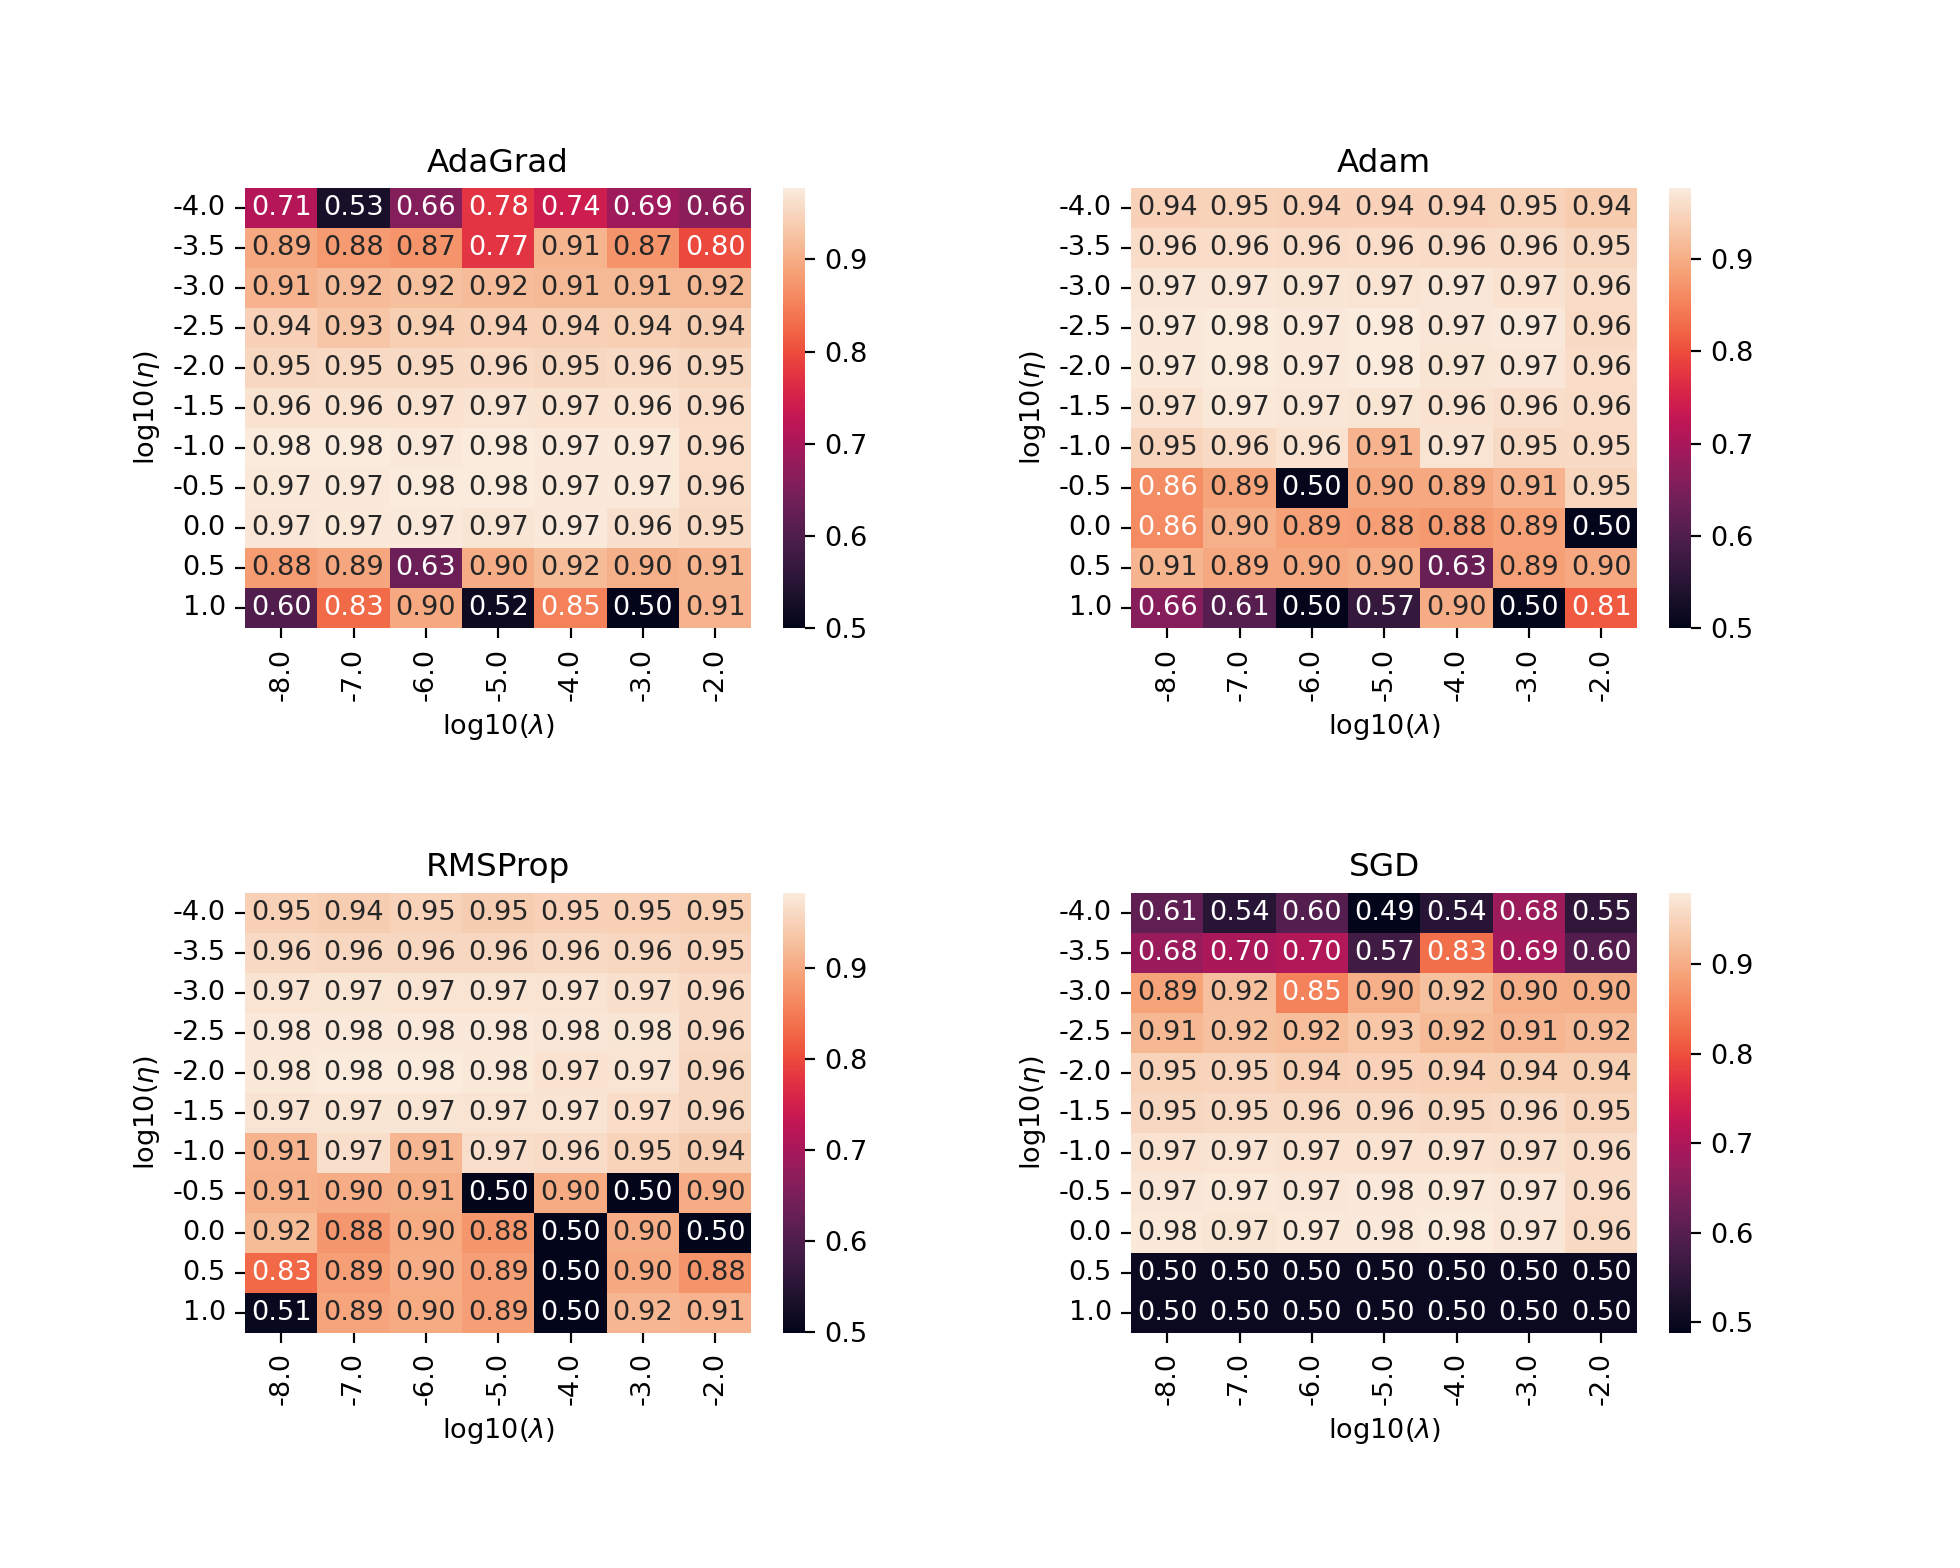
\includegraphics[scale=0.8]{nn_test_accuracy_hm}
	\caption{Shows heatmaps for the test-accuracies for the different
		models, detailing how the performance varies depending on the
		learning-rate and regularization parameter.}
	\label{nntestacchm}
\end{figure}

\begin{table}
	\centering
	\begin{tabular}{| c | c |}
		Activation function & Test-accuracy \\
		relu                & 0.9842        \\
		sigmoid             & 0.9659        \\
		swish               & 0.98055       \\
		tanh                & 0.97105       \\
		elu                 & 0.9724
	\end{tabular}
	\caption{The test-accuracies after training various neural networks on
		$10 000$ datapoints using $1$ epoch, where we for each activation
		function have optimized the learning-rate and regularization parameter.}
	\label{nnactivres}
\end{table}
\begin{table}
	\centering
	\begin{tabular}{| c | c |}
		Hidden layer sizes        & Test-accuracy \\
		(10)                      & 0.9721        \\
		(10, 10, 10)              & 0.97          \\
		(100, 100)                & 0.9845        \\
		(50, 50)                  & 0.9795        \\
		(100, 100, 100, 100)      & 0.98345       \\
		(10, 10, 10, 10)          & 0.972         \\
		(100, 100, 100, 100, 100) & 0.98215       \\
		(1000, 100, 10)           & 0.97935       \\
		(1000, 1000)              & 0.9792        \\
		(1000, 1000, 1000)        & 0.97815       \\
		(40, 100, 30)             & 0.97825
	\end{tabular}
	\caption{The test-accuracies after training various neural networks on
		$10 000$ datapoints using $1$ epoch, where we for each layer
		size have optimized the regularization parameter.}
	\label{nnsizeres}
\end{table}

\begin{figure}
	\centering
	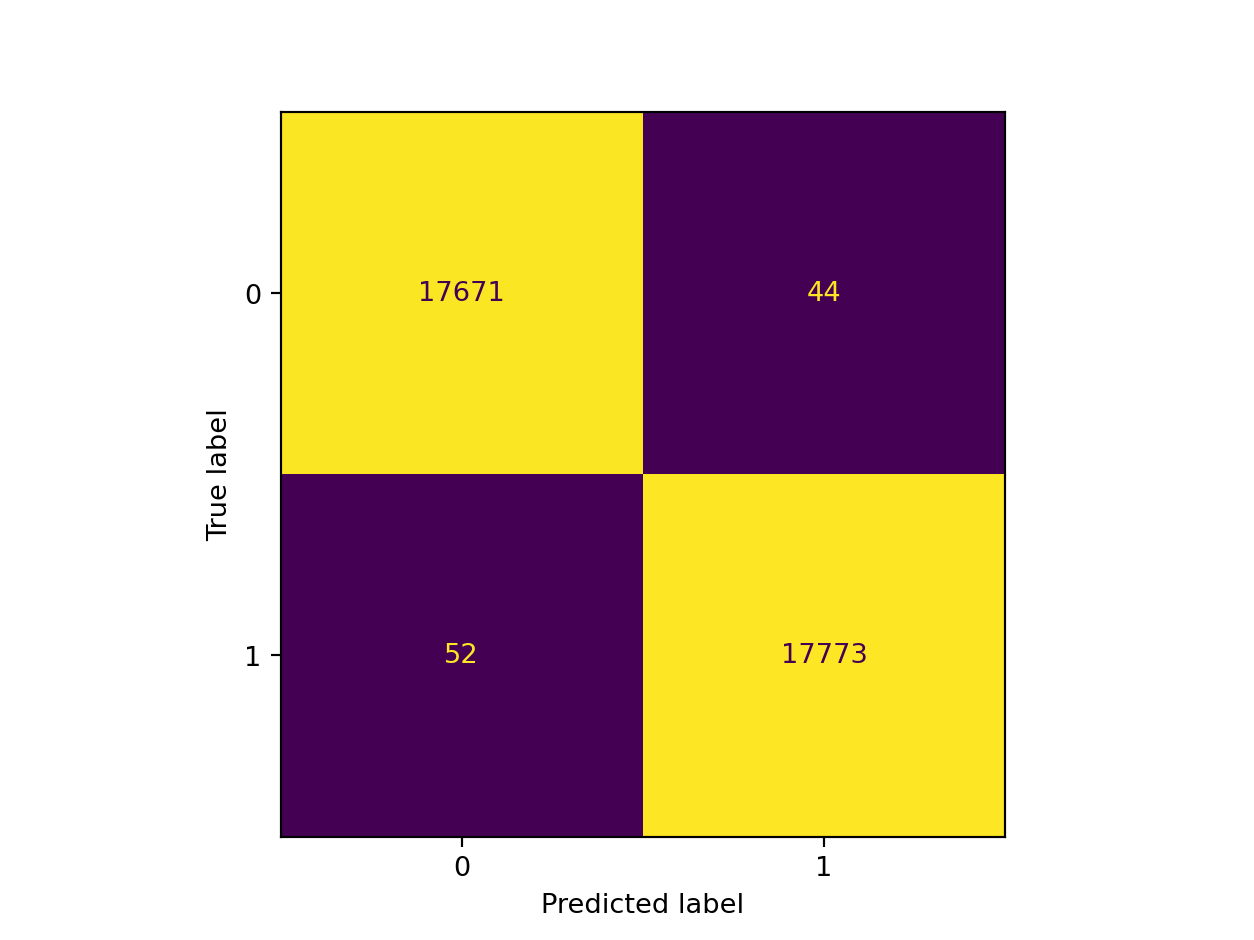
\includegraphics[scale=0.8]{nn_final_confusion_mat}
	\caption{Shows the final confusion matrix of our chosen neural network
		trained on all the training-data.}
	\label{nnconfusionmat}
\end{figure}


\subsection{Gradient boosting}
The last of our three methods was one based on gradient boosting using the
XGBoost python-library. The code for our analysis is contained in
\textbf{xgb\_creditcard.py}. Here we only tweaked the number of estimators and
the number of leaves. After optimizing these on a smaller subset of our
training and test data we get the amount of estimators giving the best results
being $360$ (giving an accuracy of $0.9945$ with the default max leaves), and
the best value of max-leaves being $6$ (yielding an accuracy of $0.9955$ with
the $360$ estimators). Figure \ref{xgbconfusionmat} shows the final confusion
matrix. We see that we are able to classify all the fraud-cases as fraud, while
also only getting $21$ false positives. Figure \ref{xgbimportance} shows the
importance-plot of each of the features. We can here see that a lot of the
features which appears to have differing distributions for the fraud and
non-fraud (looking at figure \ref{databoxplot}) cases appear to be some of the
most important, which is not particularly surprising. Finally for a
visualization of one of the weak classifiers, see figure \ref{xgbtreeplot}.

\begin{figure}
	\centering
	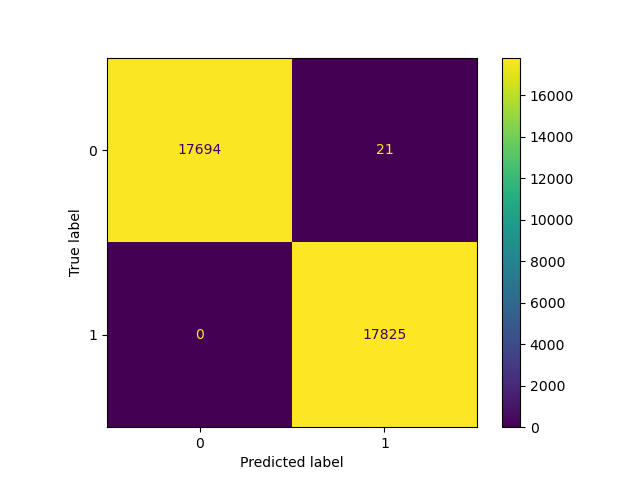
\includegraphics[scale=0.8]{xgb_final_confusion_mat}
	\caption{Shows the confusion matrix for a XGBoost gradient boosting
		model with $360$ estimators and $6$ as the max-leaves.}
	\label{xgbconfusionmat}
\end{figure}
\begin{figure}
	\centering
	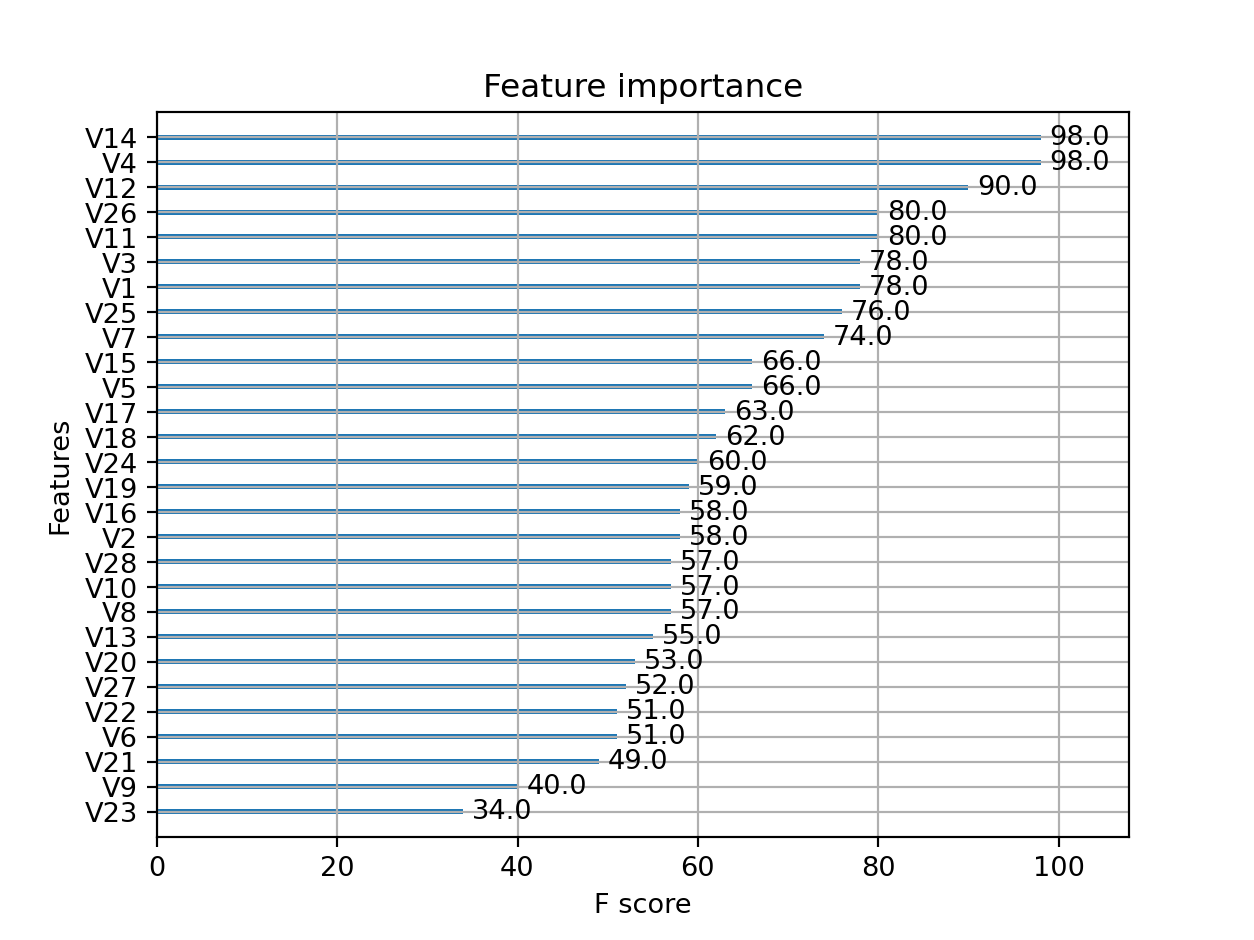
\includegraphics[scale=0.8]{xgb_final_importance}
	\caption{Shows the feature importance for our gradient boosting model.}
	\label{xgbimportance}
\end{figure}
\begin{figure}
	\centering
	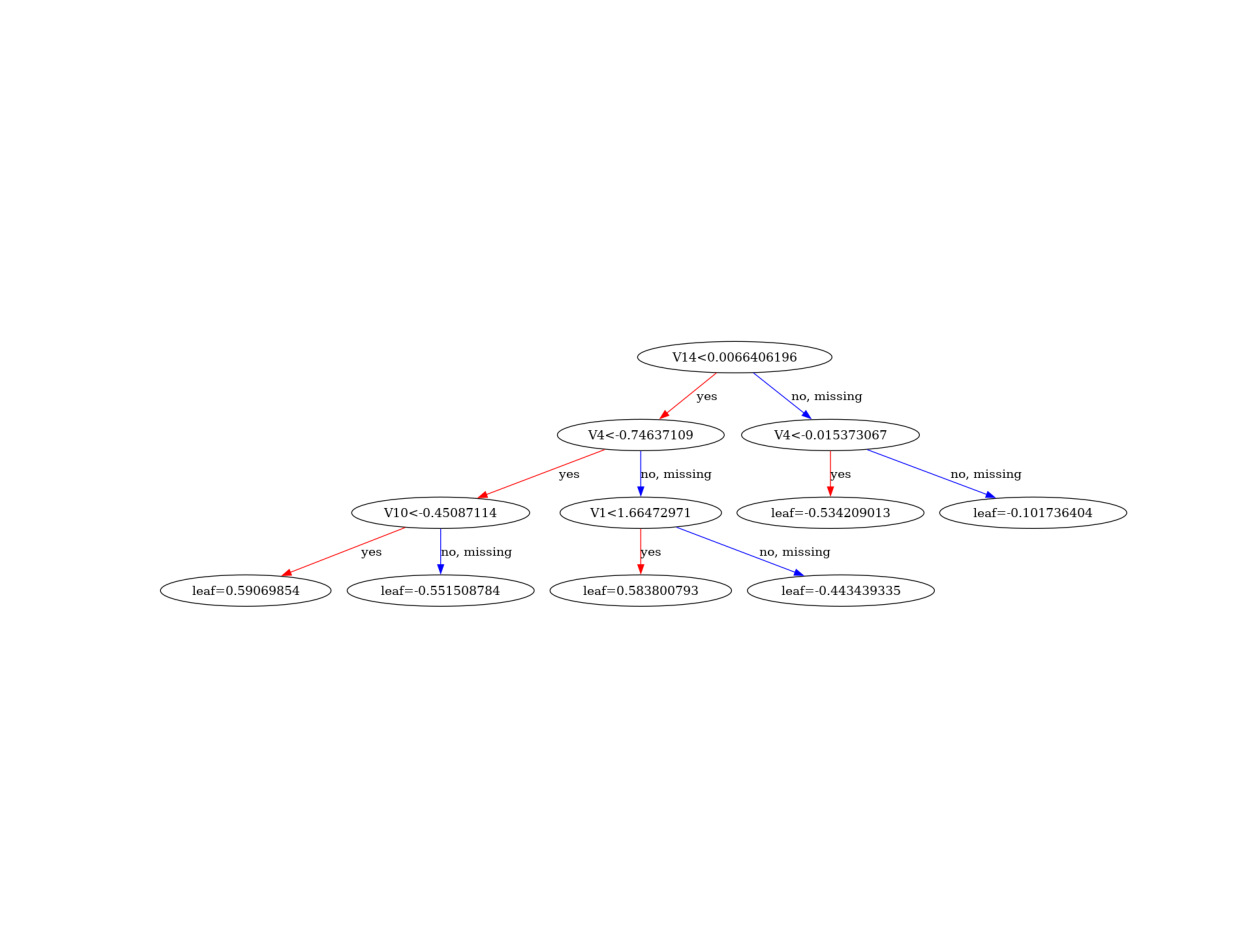
\includegraphics[scale=0.8]{xgb_final_tree_plot}
	\caption{A tree plot for one of our weak classifiers.}
	\label{xgbtreeplot}
\end{figure}

\section{Analysis}
After exploring various models and tweaking their respective hyperparameters we
then trained final models on all the training-data and evaluated the
performance on all the test-data. Table \ref{finalmodelscomparison} shows the
final accuracies of our models. As we can see, the gradient boosted trees gave
the best results for the final model. Not only that, looking at the confusion
matrices, this was also the only model which with a $0.5$ classification
threshold was able to classify all the fraud cases as fraud. Keep in mind if we
want to make sure that more or less all of the fraud cases are detected as
fraud, this is probably possible to more or less get on the neural network
model as well due by lowering the probability required for us to classify as
fraud.
\begin{table}
	\centering
	\begin{tabular}{| c | c |}
		Model                         & Test-accuracy \\
		Logistic regression (sklearn) & 0.9972        \\
		Neural network (tensorflow)   & 0.9986        \\
		Gradient boosting (XGBoost)   & 0.9994
	\end{tabular}
	\caption{The accuracy scores on the test-data for our final models.}
	\label{finalmodelscomparison}
\end{table}

One thing to keep in mind here though was that we have had to take some
shortcuts here, especially when it comes to neural networks, mostly due to the
fact that such models can become very computationally expensive. We for example
saw that some of the bigger models seemed to perform better in the neural
network case, so exploring bigger sized neural nets could change this outcome,
though such a model could take potentially hours to train properly even on
powerful hardware, which is why I have chosen to not do this here.

\section{Conclusion}

\section{Appendix}

\subsection{Project code (github)}
All the python programs described in the report and with the full source code can be
found at:
\url{https://github.com/magnouvean/ml-physics-projects/tree/main/project3/python}

\bibliography{./sources.bib}

\end{document}
